\section{Motivation}
\label{motiv:sec}

\subsection{Motivating Examples}
\label{examples:sec}

\begin{figure}[htbp]
	\centering
	\lstset{
		numbers=left,
		numberstyle= \tiny,
		keywordstyle= \color{blue!70},
		commentstyle= \color{red!50!green!50!blue!50},
		frame=shadowbox,
		rulesepcolor= \color{red!20!green!20!blue!20} ,
		xleftmargin=1.5em,xrightmargin=0em, aboveskip=1em,
		framexleftmargin=1.5em,
                numbersep= 5pt,
		language=C,
    basicstyle=\scriptsize\ttfamily,
    numberstyle=\scriptsize\ttfamily,
    emphstyle=\bfseries,
                moredelim=**[is][\color{red}]{@}{@},
		escapeinside= {(*@}{@*)}
	}
\begin{lstlisting}[]
public static void addLibraryPath(String pathToAdd) throws Exception {
  final Field usrPathsField = ClassLoader.class.(*@{\color{orange}{getDeclaredField("usr\_paths");}@*)
  usrPathsField.setAccessible(true);

  //get array of paths
  final String[] paths = (String[])usrPathsField.get(null);

  //check if the path to add is already present
  for(String path : paths) {
      if(path.equals(pathToAdd)) {
          return;
      }
  }

  //add the new path
  final String[] newPaths = Arrays.copyOf(paths, paths.length + 1);
  newPaths[newPaths.length-1] = pathToAdd;
  usrPathsField.set(null, newPaths);
}
\end{lstlisting}
        \vspace{-12pt}
        \caption{StackOverflow Post \#15409223 on Adding New Paths for
          Native Libraries at Runtime in Java}
        \label{fig:example1}
\end{figure}


Let us use a few real-world examples to explain the problem and
motivate our approach. Figure~\ref{fig:example1} displays a code
snippet in~an~answer to the StackOverflow (S/O) question 15409223 on
how~to~ {\em ``add new paths for native libraries at runtime in
  Java''}.  The code snippet serves as an illustration in the S/O
post, thus, does not contain all the details on what exceptions that
need to be handled. It contains only a throw of a generic
\code{Exception} in the method header~(\code{addLibraryPath}). From
Zhang {\em et al.}'s study~\cite{zhang-icse19}, this code snippet was
adopted by developers into their Github project named \code{armint}
(Figure~\ref{fig:example2}).~\code{armint}'s developers handle in a
\code{try-catch} block several exceptions caused~by
\code{java\-.lang\-.Class\-.get\-Declared\-Field(...)} (line 7)
according to JDK's documentation, e.g.,
\code{No\-Such\-Field\-Exception}, \code{Security\-Exception},
\code{Illegal\-Argu\-ment\-Excep\-tion}, and
\code{Illegal\-Access\-Exception} (line 24,
Figure~\ref{fig:example2}).

%In their study, Zhang {\em et al.}~\cite{zhang-icse19} have reported
%that
%Such adaptation is still largely manual~\cite{zhang-icse19}.
%Kechagia {\em et al.}~\cite{kechagia-msr14} found that 69\% of the
%methods from Android packages in their stack traces had undocumented
%exceptions in the Android APIs.
The manual adaptation on exception handling by inserting a
\code{try-catch} block is quite popular, yet not automated by any
tools~\cite{zhang-icse19}. Such manual adaptation for a code snippet
could lead to exception-related bugs, which could cause serious issues
including crashes or unstable states.
%It is not trivial for developers to memorize what API methods could
%cause exceptions and what exceptions need to be
%handled~\cite{xrank-fse20}.
Thus, it is desirable to have an automated tool to recommend proper
exception handling for such adaptation.
%in order to adapt the incomplete code snippets.
%Such a tool could recommend if a \code{try-catch} block is needed for
%the snippet, what lines need to be included in that block, and what
%exception types need to be handled.


\begin{Observation} [{\bf Exception Handling Recommendation}]
\label{ob1}
Automated recommendation to handle exceptions is desirable to
assist developers in adapting incomplete code snippets into their
codebases.
\end{Observation}

%spec, heuristic, mining, IR

As explained in Section~\ref{sec:intro},  four
categories of automated approaches have been proposed to recommend
exception
handling~\cite{xrank-fse20,barbosa-bsse12,chanchal-scam14,barbosa-tse18,barbosa-tse16}.
%--------------- Tien ---
%While early approaches were not effective in all cases due to their
%{\em heuristics}~\cite{barbosa-bsse12}, the {\em exception policies}
%are too strict in enforcing them, yet requires the rules to be encoded
%in the tools~\cite{barbosa-tse16,barbosa-saner18}. The
%state-of-the-art {\em information retrieval}-based approaches (e.g.,
%XRank/Xhand~\cite{xrank-fse20}) have been shown to outperform the
%existing approaches including the {\em mining
%  approaches}~\cite{chanchal-scam14} (which suffers the issue of
%setting a threshold for frequent occurrences).
%-----------------
However, the state-of-the-art, IR-based approaches~\cite{xrank-fse20},
which have been shown to outperform others, still have the
limitations. First, it is not trivial to pre-define a threshold for
feature matching for a retrieval, e.g., the threshold to determine the
associations between an API~call (e.g., \code{get\-Declared\-Field})
and an exception type (e.g., \code{No\-Such\-Field\-Exception}). Thus,
the pre-defined threshold affects much their effectiveness.
%
Second, relying on the lexical values of API elements' names, they
suffer the issue of ambiguous names of the APIs or exceptions in an
incomplete code snippet (e.g., the API method \code{get} at line 6 of
Figure~\ref{fig:example1} occurs in multiple libraries), which might
not be parseable for fully-qualified name resolution. Thus, this
reduces effectiveness. Finally, they consider only the associations
between an API method and an exception type, and discard the
surrounding context.
%in a \code{try-catch} block.
For example, they compute the association between the names of the API
call (e.g., \code{get\-Declared\-Field}) and the exceptions to be
handled (e.g., \code{No\-Such\-Field\-Exception},
\code{Security\-Exception}, etc.). Without the context, it is
challenging to decide the identities of the APIs and their exceptions via
only simple names.

%and the exceptions to be handled.


\begin{figure}[htbp]
	\centering
	\lstset{
		numbers=left,
		numberstyle= \tiny,
		keywordstyle= \color{blue!70},
		commentstyle= \color{red!50!green!50!blue!50},
		frame=shadowbox,
		rulesepcolor= \color{red!20!green!20!blue!20} ,
		xleftmargin=1.5em,xrightmargin=0em, aboveskip=1em,
		framexleftmargin=1.5em,
                numbersep= 5pt,
		language=C,
    basicstyle=\scriptsize\ttfamily,
    numberstyle=\scriptsize\ttfamily,
    emphstyle=\bfseries,
                moredelim=**[is][\color{red}]{@}{@},
		escapeinside= {(*@}{@*)}
	}
\begin{lstlisting}[]
/** ...
 * taken from http://stackoverflow.com/questions/15409223/
 * adding-new-paths-for-native-libraries-at-runtime-in-java
 */
private static void addLibraryPath(String pathToAdd) {
  (*@{\color{orange}{try}@*) {
    final Field usrPathsField = ClassLoader.class.(*@{\color{orange}{getDeclaredField("usr\_paths");}@*)
    usrPathsField.setAccessible(true);

    // get array of paths
    final String[] paths = (String[]) usrPathsField.get(null);

    // check if the path to add is already present
    for (String path : paths) {
      if (path.equals(pathToAdd)) {
	return;
      }
    }

    // add the new path
    final String[] newPaths = Arrays.copyOf(paths, paths.length + 1);
    newPaths[newPaths.length - 1] = pathToAdd;
    usrPathsField.set(null, newPaths);
  } (*@{\color{orange}{catch (NoSuchFieldException | SecurityException | IllegalArgumentException |    IllegalAccessException e)}@*) {
	throw new RuntimeException(e);
  }
}
\end{lstlisting}
        \vspace{-12pt}
        \caption{GitHub project \code{armint} Adapts SO Post in Figure~\ref{fig:example1}}
        \label{fig:example2}
\end{figure}



\begin{figure}[t] %[htbp]
	\centering
	\lstset{
		numbers=left,
		numberstyle= \tiny,
		keywordstyle= \color{blue!70},
		commentstyle= \color{red!50!green!50!blue!50},
		frame=shadowbox,
		rulesepcolor= \color{red!20!green!20!blue!20} ,
		xleftmargin=1.5em,xrightmargin=0em, aboveskip=1em,
		framexleftmargin=1.5em,
                numbersep= 5pt,
		language=C,
    basicstyle=\scriptsize\ttfamily,
    numberstyle=\scriptsize\ttfamily,
    emphstyle=\bfseries,
                moredelim=**[is][\color{red}]{@}{@},
		escapeinside= {(*@}{@*)}
	}
\begin{lstlisting}[]
public Object readField(Class<?> clazz, String name, Object instance) {
  (*@{\color{orange}{try}@*) {
    Field field = clazz.(*@{\color{orange}{getDeclaredField}@*)(name);
    if (!field.isAccessible()) {
       field.setAccessible(true);
    }
    return field.get(instance);
  } (*@{\color{orange}{catch (NoSuchFieldException | SecurityException | IllegalArgumentException | IllegalAccessException e)}@*) {
   throw new RuntimeException("Cannot read field value: " + clazz.getName() + "#" + name, e);
  }
}
\end{lstlisting}
        \vspace{-16pt}
        \caption{Project \code{quarkus} with same exception handling}
        \label{fig:example3}
\end{figure}


Now, consider the complete code example in Figure~\ref{fig:example3}
from the Github project named \code{quarkus}. While there are
differences between the complete code in Figure~\ref{fig:example3} and
the adapted code in Figure~\ref{fig:example2}, the lists of the handled
exceptions are the same (line 8 in Figure~\ref{fig:example3} and line
24 in Figure~\ref{fig:example2}) due to the presence of the API call
to \code{get\-Declared\-Field} in both code. This is expected because
the designers of the JDK library have the intent for developers to use
the API method \code{get\-Declared\-Field} within a \code{try-catch}
block and to handle the list of exceptions as in line 8 of
Figure~\ref{fig:example3}. Thus, to adapt the incomplete code snippet
in Figure~\ref{fig:example1}, a model could learn from the public 
repositories with complete code to suggest proper exception handling.

\begin{Observation} [{\bf Regularity of Exception Handling}]
\label{ob2}
Finding the patterns from complete code in existing code corpora could
be a good strategy for a model to {\bf learn to properly handle the
  exceptions} in adapting an (incomplete) code snippet into a
codebase.
\end{Observation}

%=======================================================
\begin{Observation} [{\bf Relations between API methods and Exceptions}]
\label{ob3}
The presence of certain API elements helps decide the exceptions that
need to be handled.
\end{Observation}

%In our motivating example,

For example, the relation between
\code{java.\-lang.\-Class.\-get\-Declared\-Field} and the exceptions
\code{No\-Such\-Field\-Exception}, \code{Secur\-ity\-Exception},
\code{Illegal\-Argument\-Exception}, and
\code{Illegal\-Access\-Exception} can be learned from the
code corpora. Thus, a model can learn to recommend those exceptions
for an incomplete code snippet involving \code{get\-Declared\-Field}.
%======================================================

%\begin{Observation} [{\bf Dependencies and Surrounding Context help resolve name ambiguity}]
%\label{ob4}
%The program dependencies among the API elements and the surrounding
%code context can help resolve the ambiguity of the names of those
%elements in incomplete code snippets.
%\end{Observation}

\begin{Observation} [{\bf Surrounding Context help resolve name ambiguity}]
\label{ob4}
%The program dependencies among the API elements and
The surrounding code context can help resolve the ambiguity of the
names of those elements in incomplete code snippets, leading to
better prediction of the handled exceptions.
\end{Observation}

For an incomplete code snippet, as explained earlier, the simple names
of the API elements (methods, fields, classes) could be ambiguous.
However, if a model can learn from the complete code the
fully-qualified names of the API elements, the surrounding context
consisting of those API elements and their program dependencies can
help a model decide the correct identities of the API elements.

%, leading to correct prediction of the handled exceptions.

\begin{figure}[htbp]
	\centering
	\lstset{
		numbers=left,
		numberstyle= \tiny,
		keywordstyle= \color{blue!70},
		commentstyle= \color{red!50!green!50!blue!50},
		frame=shadowbox,
		rulesepcolor= \color{red!20!green!20!blue!20} ,
		xleftmargin=1.5em,xrightmargin=0em, aboveskip=1em,
		framexleftmargin=1.5em,
                numbersep= 5pt,
		language=C,
    basicstyle=\scriptsize\ttfamily,
    numberstyle=\scriptsize\ttfamily,
    emphstyle=\bfseries,
                moredelim=**[is][\color{red}]{@}{@},
		escapeinside= {(*@}{@*)}
	}
\begin{lstlisting}[]
Charset charset = Charset.forName("US-ASCII");
try (BufferedReader reader = Files.newBufferedReader(file, charset)) {
    String line = null;
    while ((line = reader.readLine()) != null) {
        System.out.println(line);
    }
} catch (IOException x) {
    System.err.format("IOException: %s%n", x);
}
\end{lstlisting}
        \vspace{-12pt}
        \caption{Using \code{newBufferedReader} to read from a file}
        \label{fig:example4}
\end{figure}


\begin{figure*}[htp]
\begin{center}
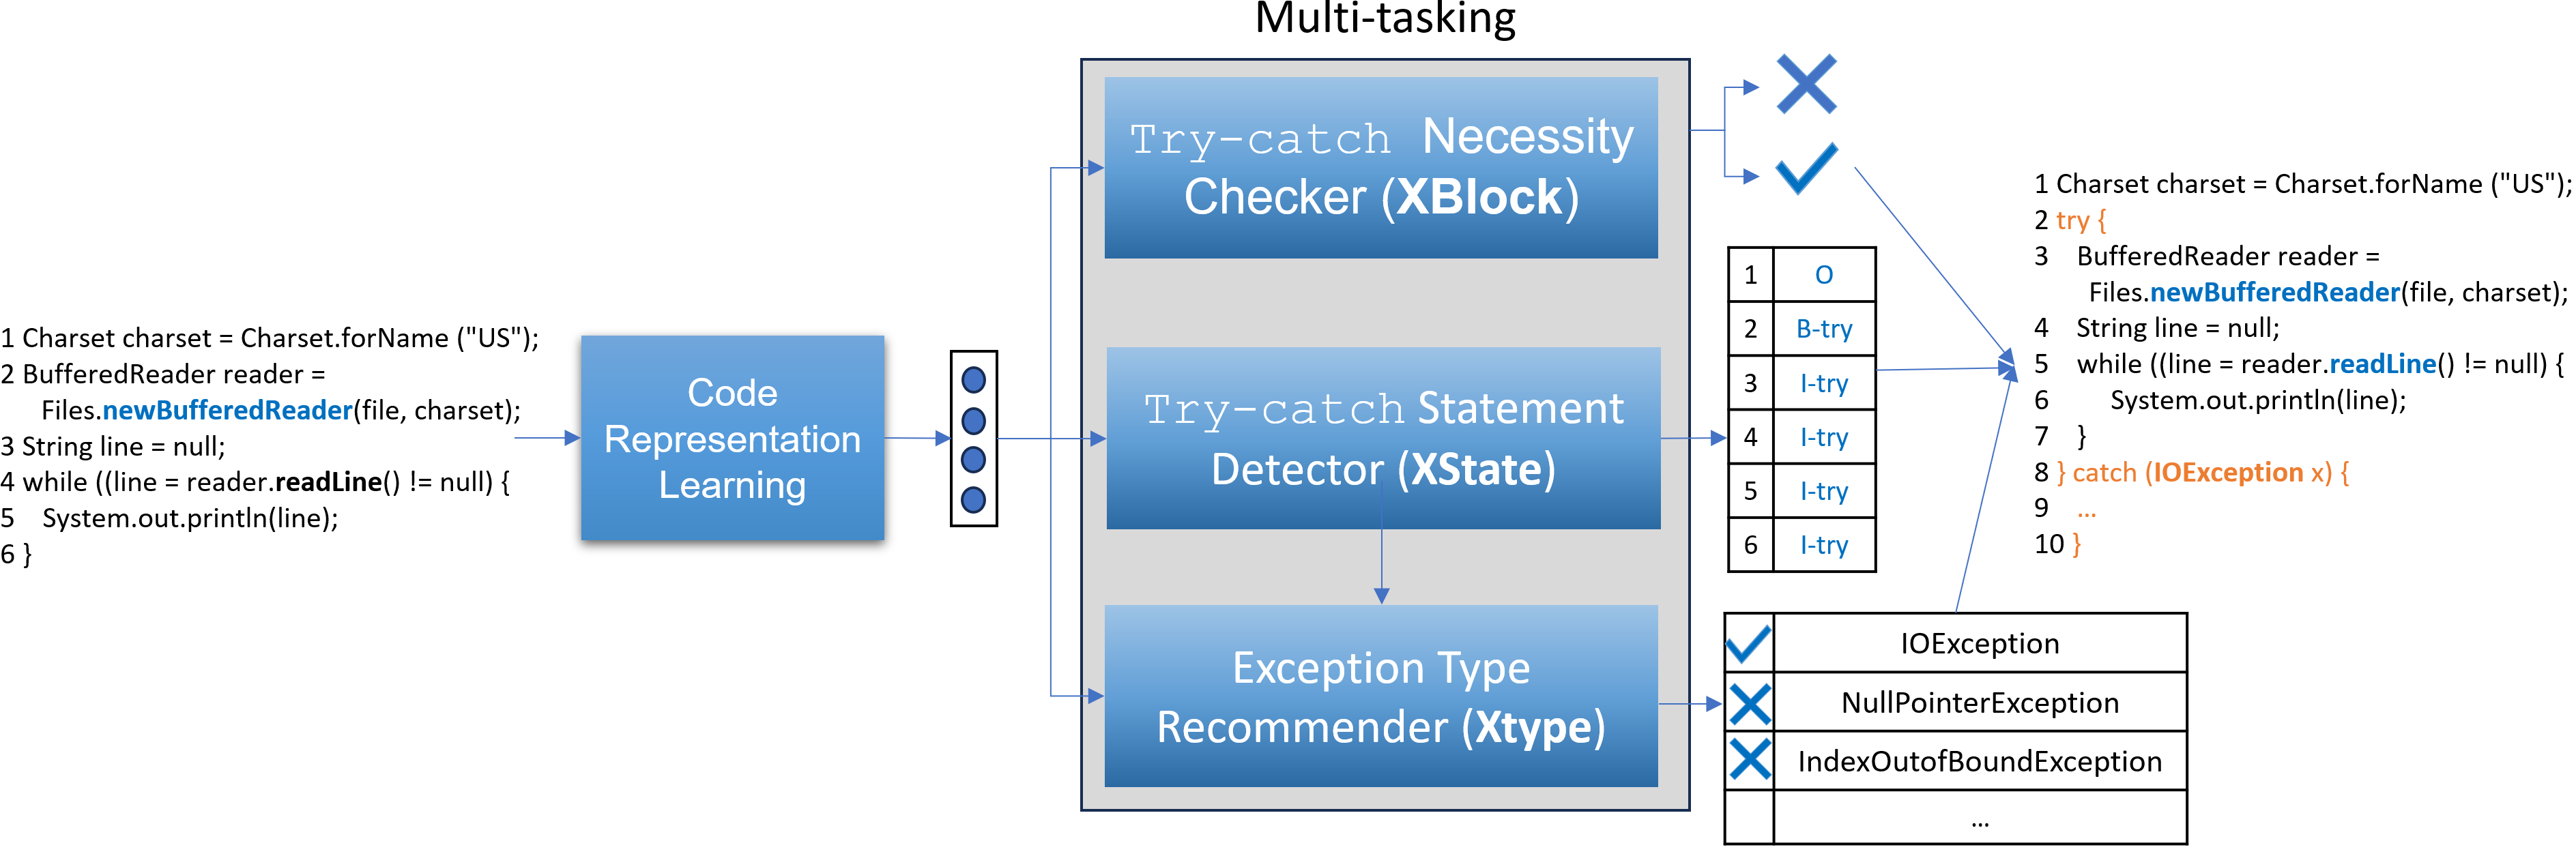
\includegraphics[width=5.6in]{overview-3.png}
\vspace{-10pt}
\caption{{\tool}: Architecture Overview}
\label{overview}
\end{center}
\end{figure*}

In Figure~\ref{fig:example1}, to derive the identities of
\code{Field} (line 2), \code{get\-Decl\-ared\-Field} (line 2),
\code{set\-Accessible} (line 3), \code{get} (line 6), etc., a model
could rely on the dependencies among them in the surrounding context.
For example, the return type of \code{get\-Declared\-Field} is
\code{Field} (thanks to line 2), which has an API method named
\code{set\-Accessible} (thanks to line 3) and another API method named
\code{get} (thanks to line 6). Considering all those dependencies among
the API elements in the context and with the knowledge learned from
the complete code, a model could decide that in the code snippet, the identity of
\code{Field} is \code{java.\-lang.\-Class.\-Field}, that of
\code{set\-Accessible} is
\code{java.\-lang.\-Class.\-Field.\-set\-Accessible}, and that of 
\code{get} at line 6 is
\code{java.\-lang.\-Class.\-Field.\-get}. The rationale is that a
model could see such dependencies among those API elements before in
a complete code in training.
%(Figure~\ref{fig:example3}).





%======================================================
For the list of statements in an incomplete code, not all of them
needs to be wrapped around in a \code{try-catch} block. For example,
considering the example of using \code{new\-Buffered\-Reader} in
Figure~\ref{fig:example4}. While the API call
\code{java.\-nio.\-file.\-new\-Bugffered\-Reader} needs to be within a
\code{try-catch} block, the statement at line 1 to retrieve the
character set does not. Moreover, the statement at line 5 with the API
call to \code{readLine} needs to be wrapped in a \code{try-catch}
block as well.






\begin{Observation} [{\bf Learn to decide what statements to be in a Try-Catch block}]
\label{ob5}
  A model can learn from the code corpora what statements need to be placed
  within a \code{try-catch} block or not.
\end{Observation}
